\documentclass[11pt]{article}

\usepackage{amsmath,amsfonts,amssymb,amsthm}
\usepackage[margin=1in]{geometry}
\usepackage{enumitem}
\usepackage{xcolor}
\usepackage[colorlinks=true, allcolors=blue]{hyperref}

\newcommand{\C}{{\mathbb{C}}}
\newcommand{\F}{{\mathbb{F}}}
\newcommand{\R}{{\mathbb{R}}}
\newcommand{\Z}{{\mathbb{Z}}}

\setlength\parindent{0pt}


\newcommand{\ket}[1]{|{#1}\rangle}
\newcommand{\bra}[1]{\langle{#1}|}
\newcommand{\braket}[2]{\<{#1}|{#2}\>}
\newcommand{\norm}[1]{\|{#1}\|}
\newcommand{\Norm}[1]{\left\|{#1}\right\|}
\newcommand{\red}[1]{{\color{red}#1}}
\theoremstyle{definition}
\newtheorem{definition}{Definition}
\newtheorem{theorem}{Theorem}[section]

\usepackage{algorithm}
\usepackage{algpseudocode}

\newcommand{\eq}[1]{(\ref{eq:#1})}
\renewcommand{\sec}[1]{Section~\ref{sec:#1}}
\usepackage{tikz}
\usetikzlibrary{positioning, shapes.geometric}
\usepackage{verbatim}
\usepackage{smartdiagram}

%%%%%%%%%%%%%%%%%%%%%%%%%%%%%%%%%%%%%%%%%%%%%%%%%%%%%%%%%%%%%%%%%%%%%%%%%%%%%%
\begin{document}

\title{Numerically solving time evolution partial differential equations by variational quantum circuits:  Final Report}

\author{Yang Lv}

\date{}
\maketitle

\begin{abstract}
We explain how a family of time evolution PDEs which have deep connection with stochastic process can be simulated using variational quantum imaginary time evolution. We also introduce machine learning algorithms to solve the equations and make comparison to the quantum algorithm. We  conclude that more work needs to be done to claim quantum algorithms can overcome curse of dimensionality, point out problems in the algorithm and propose some future aspects.
\end{abstract}

%%%%%%%%%%%%%%%%%%%%%%%%%%%%%%%%%%%%%%%%%%%%%%%%%%%%%%%%%%%%%%%%%%%%%%%%%%%%%%

\section{Introduction}\label{sec:intro}
\paragraph{Motivations.}
Partial differential equations(PDEs) are ubiqitous in natural, social and information science. These equations describe the fundamental laws of nature  and have been studied by Mathematicians intensively, on the theoretical properties and numerical approximation algorithms. Some well-known PDEs include Navier-Stokes equations, Schrödinger equation and Hamilton-Jacobi-Bellman equation.  Today the majority of supercomputing resources in the world are dedicated to finding accurate numerical simulation of PDEs. Successful numerical algorithms developed include finite difference methods, finite element methods and spectral methods. These methods have theoretical guarantees (bounds on error and guarantee of convergence) and thus are successfully applied to engineering and scientific problems. However, despite their great success, these traditional methods face some fundamental challenges. The essential difficulty is  the curse of dimensionality\cite{e_machine_2020}, which describes the phenomenon that with the dimension $d$ of the PDE grows to hundreds and beyond, to get a fixed overall error $\epsilon$, you need at least $\Omega(C^d)$ memory to store the approximation information for some constant $C$, which is infeasible. Other typical challenges include programming with complex and irregular boundary conditions, and dealing with singularities.\\

In recent years, machine learning has seen great success in the field of computer vision and natural language processing. The problems these fields concerns, like image recognition (approximating a map from $\R^{n\times n \times 3}$ to $\left[1,...M \right]$ where $M$ is the number of categories and $n$ is the resolution of image) are very high-dimensional. Computational mathematicians and computer scientists are thus inspired and used the deep neural networks to develop some successful algorithms to solve forward and inverse problems in PDE, including PINNs\cite{raissi_physics_2017}, deep BSDE\cite{han_solving_2018}, Fourier Neural operators\cite{li_fourier_2021} etc. Althogh these algorithms do work empirically, due to the black-box nature of deep learning, they are not guaranteed to converge theoretically, and users cannot set the accuracy as needed.\\

Another rising field\cite{childs_high-precision_2021}\cite{leong_variational_2022}\cite{yuan_theory_2019}, which has attracted less attention from the computational math community is quantum computing. Quantum computing utilizes the superposition of quantum states and uses hardware implementations of unitary operations to do computation. Because the state space of $n$ qubits is  $\C^{\otimes2^n}$, it is quite reasonable to expect it solves the curse of dimensionality entirely. Indeed, quantum algorithms are proven to have exponential speedup in some problems, including unstructured search and solving linear system of equations. Quantum computing has been criticized of existing much theoretically and cannot be really implemented, at least in a near future. However, near-term quantum computers are believed to be able to compute with few qubits and short sequence of quantum gates. Therefore, it is reasonable and important to investigate quantum computers for solving (high dimensional) PDEs.\\

A family of parabolic PDEs enjoy some very beautiful mathematical properties, namely they are deeply connected with stochastic process which can be modeled by stochastic differential equations by the Feynman-Kac formula\cite{e_applied_2019}. This opens a door for machine learning to simulate the solution. On the other hand, after certain transformations, the PDEs can be transformed to have similar form with Schrödinger equation, making it possible to use quantum simulation techniques to approximate the solution. Therefore, this type of PDEs are great examples through which we can explore the possibility of using the emerging techniques to solve PDEs.\\

We will follow a newly released paper \cite{alghassi_variational_2022} accepted in \textit{Quantum} to understand the quantum computing algorithm for the  PDE, with a comparison between the machine learning way to address it. We will differ slightly from the structure of and make necessary simplifications. Machine learning and quantum computing are among the most powerful tools we own to deal with high dimension  Is machine learning really the default way of coping with high dimensional problems in PDEs? Maybe we should also pay more attention to quantum computing. 



\paragraph{Main results.}
We will mainly investigate the quantum algorithm described in .We provide here a flow illustration of the quantum algorithm, the detailed definition and meaning of each step will be explained in the following sections. \\

\textit{Variational quantum algorithm for PDE}

\smartdiagramset{
                    border color=none,
                    back arrow disabled=true
                }
\smartdiagram[flow diagram:horizontal]{Acquire  operator, Discrete  \& decompose operator, Ansatz design,  Initialization, Solve ODE \& update parameters, Readout solution}



\paragraph{Organization.}
The result of the paper is organized as follows. In Section $2$, we present the preliminary knowledge of PDEs, Brownian motion, stochastic differential equations, and Feynman-Kac formula. In Section $3$, we discuss the quantum algorithm for solving the PDE and its analysis and briefly introduce the machine learning methods for solving the PDE. We make discussion on the advantages and shortcomings of the methods in Section $4$. Finally, a conclusion is presented in Section $5$.

%%%%%%%%%%%%%%%%%%%%%%%%%%%%%%%%%%%%%%%%%%%%%%%%%%%%%%%%%%%%%%%%%%%%%%%%%%%%%%

\section{Preliminaries}\label{sec:prelim}
We first define partial differential equations.
\begin{definition}
 A PDE\cite{evans_partial_1998} in a single unknown $u$ is a functional equation involving $u$ and its partial derivatives. All such equations have the form of
$$\quad F\left(u, u_{x^1}, \cdots, u_{x^n}, u_{x^1 x^1}, \cdots, u_{x^{i_1} \ldots x^{i_N}}, x^1, x^2, \cdots, x^n\right)=0, \quad i_1, \cdots, i_N \in\{1,2, \cdots, n\}
$$ 
for some function $F$.
Here $N$ is called the order of the PDE. $N$ is the maximum number of derivatives appearing in the equation.    
\end{definition}
A PDE is itself is not enough to determine the evolution of the system. Certain initial condition or boundary value condition must also be provided to fully determine the system. The type of boundary condition has a huge impact on the numerical algorithm, but we will omit the discussion of them in this paper and assume periodic boundary condition througuout.\\

Let's start with the (standard) Brownian motion, also known as the Wiener process in mathematical literature. Let $\left( \Omega,\mathcal{F},\mathbb{P}\right)$ be a probability space.
\begin{definition}
Brownian motion $W_t=W(t)$ with $t \geq 0$ is a continuous stochastic process that satisfies the following characteristics:\\
\begin{enumerate}
    \item $W(0)=0$ almost surely;
    \item $W(t+u)-W(t)$ is independent of $\sigma(W(s): s \leq t)$ for $u \geq 0$, where $\sigma$ denotes the sigma algebra generated by $W(s)$, which means $W(t)$ has independent increments;
    \item $W(t+u)-W(t)$ is normally distributed with mean 0 and variance $u$, i.e. $W(t+u)-W(t) \sim \mathcal{N}(0, u)$, that is $W(t)$ has Gaussian increments;
    \item $W(t)$ is a continuous function of $t$, i.e. $t \rightarrow W(t, \omega)$ is continuous in $t$ for all $\omega \in \Omega$.
\end{enumerate}

\end{definition}

With Brownian motion defined, we can move to stochastic differential equations. Suppose we have a filtered probability space $\left( \Omega,\mathcal{F},\mathbb{P}\right)$.
\begin{definition}
    A general stochastic differential equation(SDE) is of the form
$$
\mathrm{d} \textbf{X}_t=\mu\left(\textbf{X}_t, t\right) \mathrm{d} t+\sigma\left( \textbf{X}_t, t\right) \mathrm{d} W_t,
$$
where $W$ denotes a Wiener process (standard Brownian motion). This equation should be interpreted as an informal way of expressing the corresponding integral equation
$$
\textbf{X}_{t+s}-\textbf{X}_t=\int_t^{t+s} \mu\left(X_u, u\right) \mathrm{d} u+\int_t^{t+s} \sigma\left(X_u, u\right) \mathrm{d} W_u
$$
\end{definition}

Here, filtered probability space, integral of stochastic functions and integral with respect to Brownian motion are too technical and we choose not to go into details. Interested readers can refer to \cite{e_applied_2019}. Intuitively, SDEs are very similar to ODEs, and $\mathrm{d} t$, $\mathrm{d} B_t$ can be understood heuristically.\\

Finally, let's introduce the Feynman-Kac formula, which is the bridge between SDEs and coresponding time-evolution PDEs.
\begin{theorem}($1$D Feynamn-Kac)
Consider a stochastic differential equation
$$
d X_t=\mathfrak{b}\left(X_t, t\right) d t+\sqrt{2 \mathfrak{a}\left(X_t, t\right)} d W_t
$$ on probability space $(\Omega, \mathcal{F}, \mathbb{P})$.

Here $\mathfrak{a}$ and $\mathfrak{b}$ are  analytic functions with $\mathfrak{a}>0$ and with condition $X_t=x$.  Let $\mathfrak{f}: \mathbb{R} \rightarrow \mathbb{R}$ be an analytic function. For a Borel-measurable function $\psi: \mathbb{R} \rightarrow \mathbb{R}$, define $u: \mathbb{R} \times[0, T] \rightarrow \mathbb{R}$ by setting
$$
\begin{aligned}
u(x, t)= & \mathbb{E}\left[\int_t^T \exp \left(-\int_t^s \mathfrak{c}\left(X_\tau, \tau\right) d \tau\right) \mathfrak{f}\left(X_s, s\right) d s\right. \\
& \left.+\exp \left(-\int_t^T \mathfrak{c}\left(X_\tau, \tau\right) d \tau\right) \psi\left(X_T\right) \mid X_t=x\right]
\end{aligned}
$$
Under suitable technical condition,
the function $u$ is defined for $0<T-t<\frac{1}{2} \delta$ and $x \in \mathbb{R}$, and has derivatives of all orders. In particular, it belongs to the class $\mathcal{C}^{2,1}(\mathbb{R} \times(0, T))$. Then we have $u$ satisfies the following partial differential equation
$$
\left\{\begin{array}{l}
\frac{\partial u}{\partial t}+\mathfrak{a}(x, t) \frac{\partial^2 u}{\partial x^2}+\mathfrak{b}(x, t) \frac{\partial u}{\partial x}-\mathfrak{c}(x, t) u+\mathfrak{f}(x, t)=0, \quad \text { for } \quad t<T \\
u(x, T)=\psi(x)
\end{array}\right.
$$



\end{theorem}

\begin{theorem}(General Feynmac-Kac)
Let $D \in \mathbb{N}$ and $N \in \mathbb{N}$ and consider a $D$-dimensional stochastic process
$$
\mathbf{X}_t=\left(X_t^1, X_t^2, \cdots, X_t^D\right)^T
$$
governed by an $N$-dimensional Brownian motion
$$
\mathbf{W}_t=\left(W_t^1, W_t^2, \cdots, W_t^N\right)^T,
$$
whose time evolution is given by the following system of SDEs:
$$
d X_t^i=\mu_i\left(\mathbf{X}_t, t\right) d t+\sum_{\ell=1}^N \sigma_{i \ell}\left(\mathbf{X}_t, t\right) d W_t^{\ell}, \quad \text { for } \quad i=1,2, \cdots, D .
$$
To write in a compact form,
$$
\begin{cases}d \mathbf{X}_t & =\mu\left(\mathbf{X}_t, t\right) d t+\boldsymbol{\Sigma} \cdot d \mathbf{W}_t, \\ \mathbf{X}_0 & =\mathbf{x}_0,\end{cases}
$$
where $\mathbf{X}_t, \mathbf{x}_0$ and $\mu$ are in $\mathbb{R}^D, \mathbf{W}_t$ is in $\mathbb{R}^N$, and $\boldsymbol{\Sigma}$ is the $\mathbb{R}^{D \times N}$ matrix with elements $\sigma_{i k}\left(\mathbf{X}_t, t\right)$. \\
Define differential operator $\mathcal{G}$ as follows:
$$
\mathcal{G}=\frac{1}{2} \sum_{i=1}^D \sum_{j=1}^D \sum_{\ell=1}^N \sigma_{i \ell}\left(\mathbf{X}_t, t\right) \sigma_{j \ell}\left(\mathbf{X}_t, t\right) \frac{\partial^2}{\partial x_i \partial x_j}+\sum_{i=1}^D \mu_i\left(\mathbf{X}_t, t\right) \frac{\partial}{\partial x_i} .
$$
Denote by $\left(\boldsymbol{\Sigma} \boldsymbol{\Sigma}^{\mathbf{T}}\right)_{i j}=\sum_{\ell=1}^N \sigma_{i \ell}\left(\mathbf{X}_t, t\right) \sigma_{j \ell}\left(\mathbf{X}_t, t\right)$.  Now set
$$
u(\mathbf{x}, t)=\mathbb{E}\left[\exp \left(-\int_0^t r\left(\mathbf{X}_s, s\right) d s\right) \psi\left(\mathbf{X}_t\right) \mid \mathbf{X}_t=\mathbf{x}\right]
$$
for some well-behaved function $\psi$. The function $u$  satisfies the diffusion PDE
$$
\frac{\partial u}{\partial t}=\mathcal{G} u-r u, \quad t>0
$$

as well as the initial condition $u(\mathbf{x}, 0)=\psi(\mathbf{x})$. 
\end{theorem}
%%%%%%%%%%%%%%%%%%%%%%%%%%%%%%%%%%%%%%%%%%%%%%%%%%%%%%%%%%%%%%%%%%%%%%%%%%%%%%

\section{Algorithm}
\subsection{Quantum algorithm}
We now go detail into the quantum algorithm.
\subsubsection{Operator discretization}
(Classical and quantum) computers cannot manipulate  differential operator $\mathcal{G}$ acting on infinite dimensional function space. Using finite difference approximation, one can approximate $\mathcal{G}$ by operators acting on finite dimensional state space. By Taylor expansion,
$$
\begin{aligned}
& \frac{\partial u\left(x_{i_1}, x_{i_2}, \cdots, x_{i_D}, t\right)}{\partial x_{i_d}} \approx \frac{u_{\mathbf{i}+\mathbf{e}_d}-u_{\mathbf{i}-\mathbf{e}_d}}{2 \Delta x_{i_d}}, \\
& \frac{\partial^2 u\left(x_{i_1}, x_{i_2}, \cdots, x_{i_D}, t\right)}{\partial x_{i_d}^2} \approx \frac{u_{\mathbf{i}+\mathbf{e}_d}-2 u_{\mathbf{i}}+u_{\mathbf{i}-\mathbf{e}_d}}{\Delta x_{i_d}^2}, \\
&
\end{aligned}
$$
Discretize the domain of the PDE (which, without loss of generality, can be assumed to be a hypercube in $D$ dimension) by uniform grids. See below figure for an illustration (taken from \cite{alghassi_variational_2022}).

\begin{center}
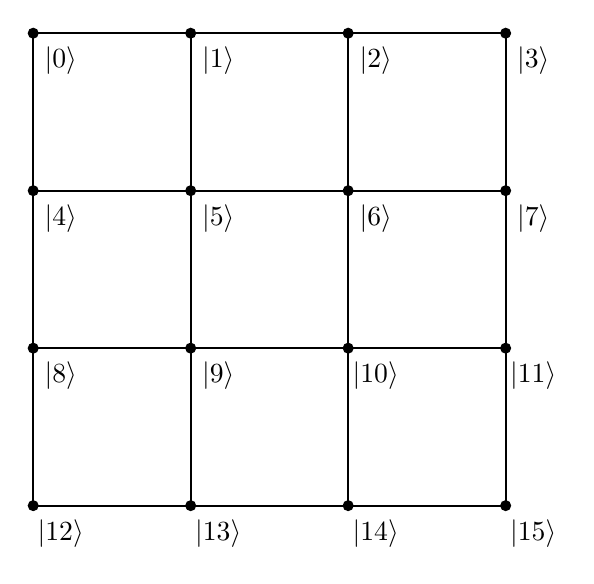
\begin{tikzpicture}
\label{theMaindiag}
\draw[step=2cm, black, thick] (0,0) grid (6,6);
\foreach \x in {0, 2, 4, 6}
    \foreach \y in {0, 2, 4, 6}
        \fill (\x, \y) circle [radius=2pt];
\draw(0.35, 5.65) node{$|0\rangle$};
\draw(2.35, 5.65) node{$|1\rangle$};
\draw(4.35, 5.65) node{$|2\rangle$};
\draw(6.35, 5.65) node{$|3\rangle$};
\draw(0.35, 3.65) node{$|4\rangle$};
\draw(2.35, 3.65) node{$|5\rangle$};
\draw(4.35, 3.65) node{$|6\rangle$};
\draw(6.35, 3.65) node{$|7\rangle$};
\draw(0.35, 1.65) node{$|8\rangle$};
\draw(2.35, 1.65) node{$|9\rangle$};
\draw(4.35, 1.65) node{$|10\rangle$};
\draw(6.35, 1.65) node{$|11\rangle$};
\draw(0.35,-0.35) node{$|12\rangle$};
\draw(2.35,-0.35) node{$|13\rangle$};
\draw(4.35,-0.35) node{$|14\rangle$};
\draw(6.35,-0.35) node{$|15\rangle$};
\end{tikzpicture}
\end{center}


Suppose resolution on each side is $n_m$, and we have in total $n_q$ qubits available. A simple relation is $$n_m=2^{\frac{n_q}{D}}$$
We can write
$$
\tilde{\mathcal{G}}=\sum_{i_1=0}^{n_m-1} \sum_{i_2=0}^{n_m-1} \cdots \sum_{i_D=0}^{n_m-1} \sum_{j_1=0}^{n_m-1} \sum_{j_2=0}^{n_m-1} \cdots \sum_{j_D=0}^{n_m-1}[\hat{\mathcal{G}}]_{i_1, i_2, \cdots, i_D, j_1, j_2, \cdots, j_D}|\mathbf{i}\rangle\langle\mathbf{j}|
$$ for suitable complex numbers $[\hat{\mathcal{G}}]_{i_1, i_2, \cdots, i_D, j_1, j_2, \cdots, j_D}$ .
\subsubsection{Variational quantum imaginary time evolution (varQITE)}
We now turn to the core of the algorithm. Transform the diffusion PDE
$$
\frac{\partial u}{\partial t}=\mathcal{G} u-r u, \quad t>0
$$
to Schrödinger-type equation
$$
\frac{\partial}{\partial t}|\psi(t)\rangle=-i \tilde{\mathcal{G}}|\psi(t)\rangle \quad \text { where } \quad \tilde{\mathcal{G}}=\mathcal{G}-r \mathbb{I}
$$
by introducing an appropriate Wick rotation $\xi=-i \tau$.\\

This PDE differs from the Schrödinger by a factor of $i$, which makes all the difference. For instance, the resulting $|\psi(t)\rangle$ may not be unitary. To simulate this PDE, we have to use a newly developed tool, the variational quantum imaginary time evolution (varQITE)\cite{yuan_theory_2019}, was originally developed for problems in quantum chemistry to compute ground-state energy, etc. \\

Consider the general equation
$$
\frac{\partial}{\partial t}|\tilde{\psi}(\mathbf{x}, t)\rangle=\mathcal{E}(t)|\tilde{\psi}(\mathbf{x}, t)\rangle
$$
where $\mathcal{E}(t)$ is now a linear time-dependent not necessarily Hermitian operator, the dynamical evolution of $|\tilde{\psi}(\mathbf{x}, t)\rangle$ can be simulated by introducing an ansatz $|\tilde{v}(\boldsymbol{\theta}(t))\rangle=$ $\alpha(t)|v(\boldsymbol{\theta}(t))\rangle$ of the form $|v(\boldsymbol{\theta}(t))\rangle=\mathbf{G}(\boldsymbol{\theta}(t))|0\rangle^{\otimes n}$ where $\alpha(t)$ is a parameter of the ansatz that scales the $\ell_2$ normalized quantum state to the desired scale and $\mathbf{G}(\boldsymbol{\theta}(t))=$ $\prod_{i=1}^N \mathbf{G}_i\left(\theta_i(t)\right)$ is the product of $N$ parametric unitaries $\mathbf{G}_i$, each composed of one parametric rotation gates $e^{i \theta_k \mathfrak{G}_k}$ with $\mathfrak{G}_k^{\dagger}=\mathfrak{G}_k$.\\

It's important to note that the ansatz, which is the correspondence of $|\tilde{\psi}(\mathbf{x}, t)\rangle$ and $|v(\boldsymbol{\theta}(t))\rangle$ described by the quantum gates $\mathfrak{G}_k$ need to be \textbf{handy crafted}, and is highly nontrivial and vital to success of the algorithm. Initialization also needs to be done here.\\

After designing the ansatz, the desired value of the parameters is then determined by McLachlan's variational principle, i.e.
$$
\delta \| \frac{\partial}{\partial t}|\tilde{v}(\boldsymbol{\theta}(t))\rangle-\mathcal{E}(t)|\tilde{v}(\boldsymbol{\theta}(t))\rangle \|=0
$$
which reads as the Euler-Lagrange-type of ODEs
$$
\boldsymbol{M} \dot{\boldsymbol{\theta}} = \boldsymbol{V}
$$
that is,
$$
\sum_{j=0}^N M_{k, j} \dot{\theta}_k=V_k, \quad \text { for each } \quad k=0,1, \cdots N .
$$
Here the elements of the matrix $M_{k, j}$ are given by
$$
M_{k, j}=\operatorname{Re}\left(\alpha^2(t) \frac{\partial\langle v(\boldsymbol{\theta}(t))|}{\partial \theta_k} \frac{\partial|v(\boldsymbol{\theta}(t))\rangle}{\partial \theta_j}\right), \quad \text { for } \quad k, j \neq 0,
$$
$$
M_{0, j}=M_{j, 0}=\alpha(t) \operatorname{Re}\left(\langle v(\boldsymbol{\theta}(t))| \frac{\partial|v(\boldsymbol{\theta}(t))\rangle}{\partial \theta_j}\right), \quad \text { for } \quad j>0,
$$
depending on the ansatz and
$$
V_k=\alpha(t) \operatorname{Re}\left(\frac{\partial\langle v(\boldsymbol{\theta}(t))|}{\partial \theta_k} \mathcal{E}|v(\boldsymbol{\theta}(t))\rangle\right), \quad \text { for } \quad k>0,
$$
$$
 V_0=\operatorname{Re}(\langle v(\boldsymbol{\theta}(t))|\mathcal{E}| v(\boldsymbol{\theta}(t))\rangle).
 $$
 depending on the operator.\\
 
 Finally, use forward-Euler Scheme to solve this ODE gives parameter update rule:
$$
\boldsymbol{\theta}(\tau+\delta \tau) \sim \boldsymbol{\theta}(\tau)+\dot{\boldsymbol{\theta}} \delta \tau=\boldsymbol{\theta}(\tau)+\mathbf{M}^{-1}(\tau) \cdot \mathbf{V} \delta \tau
$$
\subsubsection{Operator decomposition}
To realize the operator $\mathcal{E}$ which in our problem is $ \tilde{\mathcal{G}}$, we need to implement it as linear combination of implementable unitaries.
$$
\mathcal{E}(t)=\sum_{h=1}^H \lambda_h U_h,
$$
where $\lambda_h \in \mathbb{C}$ and $U_h$ is an easily implementable unitary operator made of Pauli operators. This requires an evaluation of $\mathcal{O}\left(N^2\right)+\mathcal{O}(N H)$ different quantum circuits. The whole implementation is demonstrated possible but the exact process is very tedious and we will omit it.
\subsubsection{Quantum embedding}
Quantum embedding is the process of embedding the unstructured data into quantum states. Here, the solution to the PDEs are probability distributions and therefore preserve $ell_1$ norm instead of $ell_2$ norm. We do the embedding by letting
$$
|\tilde{\psi}(t)\rangle=\alpha(t)|\psi(t)\rangle, \quad|\tilde{\psi}(t)\rangle=\sum_{i=0}^{2^n-1} p_i(t)|i\rangle \quad \text { with } \quad p_i(t)=u\left(x_i, t\right)=\mathbb{P}\left[X(t)=x_i\right],
$$
$$
\alpha(t)=\left(\sum_{i=0}^{2^n-1} p_i^2(t)\right)^{1 / 2},
$$
and
$$
|\psi(t)\rangle=\sum_{i=0}^{2^n-1} \sqrt{p_i(t)}|i\rangle .
$$
This establishes a bijection between normalized and unnormalized states.
\subsubsection{Error analysis}
Unfortunately, the authors fail to provide an overall error analysis. And to the best of our knowledge, it doesn't exist in literature as well. A relevant result is a  posterior error control of varQITE given in \cite{zoufal_error_2021}. \\
\begin{theorem}
    Bures metric is defined as
$$
\begin{aligned}
& B\left(\left|\psi_t^\omega\right\rangle\left\langle\psi_t^\omega|,| \psi_t^*\right\rangle\left\langle\psi_t^*\right|\right)= \\
& \sqrt{\left\langle\psi_t^\omega \mid \psi_t^\omega\right\rangle+\left\langle\psi_t^* \mid \psi_t^*\right\rangle-2\left|\left\langle\psi_t^\omega \mid \psi_t^*\right\rangle\right|}
\end{aligned}
$$

 For $T>0$ and $\varepsilon_0=0$, let $\left|\psi_T^*\right\rangle$ be the exact solution to the evolution equation and $\left|\psi_T^\omega\right\rangle$ be the simulation implemented using $\operatorname{VarQITE}$. Then
$$
B\left(\left|\psi_T^*\right\rangle\left\langle\psi_T^*|,| \psi_T^\omega\right\rangle\left\langle\psi_T^\omega\right|\right) \leq \epsilon_T,
$$
for $\epsilon_T=\int_0^T \dot{\varepsilon}_t \mathrm{~d} t$, where
$$
\begin{aligned}
\varepsilon_{t+\delta_t}=\delta_t \| & \left.\| e_t\right\rangle \|_2+\delta_t \zeta\left(\omega_t, \epsilon_t\right) \\
& +\sqrt{2+2 \delta_t \zeta\left(\omega_t, \epsilon_t\right)-2 \chi\left(\omega_t, \epsilon_t\right)},
\end{aligned}
$$
allows us to define
$$
\begin{aligned}
\dot{\varepsilon}_t= & \lim _{\delta_t \rightarrow 0} \frac{\varepsilon_{t+\delta_t}-\varepsilon_t}{\delta_t} \\
= & \|\left|e_t\right\rangle \|_2+\zeta\left(\boldsymbol{\omega}_{\boldsymbol{t}}, \epsilon_t\right) \\
& +\lim _{\delta_t \rightarrow 0} \frac{\sqrt{2+2 \delta_t \zeta\left(\boldsymbol{\omega}_{\boldsymbol{t}}, \epsilon_t\right)-2 \chi\left(\boldsymbol{\omega}_t, \epsilon_t\right)}-\varepsilon_t}{\delta_t}
\end{aligned}
$$.
\end{theorem}
\begin{figure}
\centering
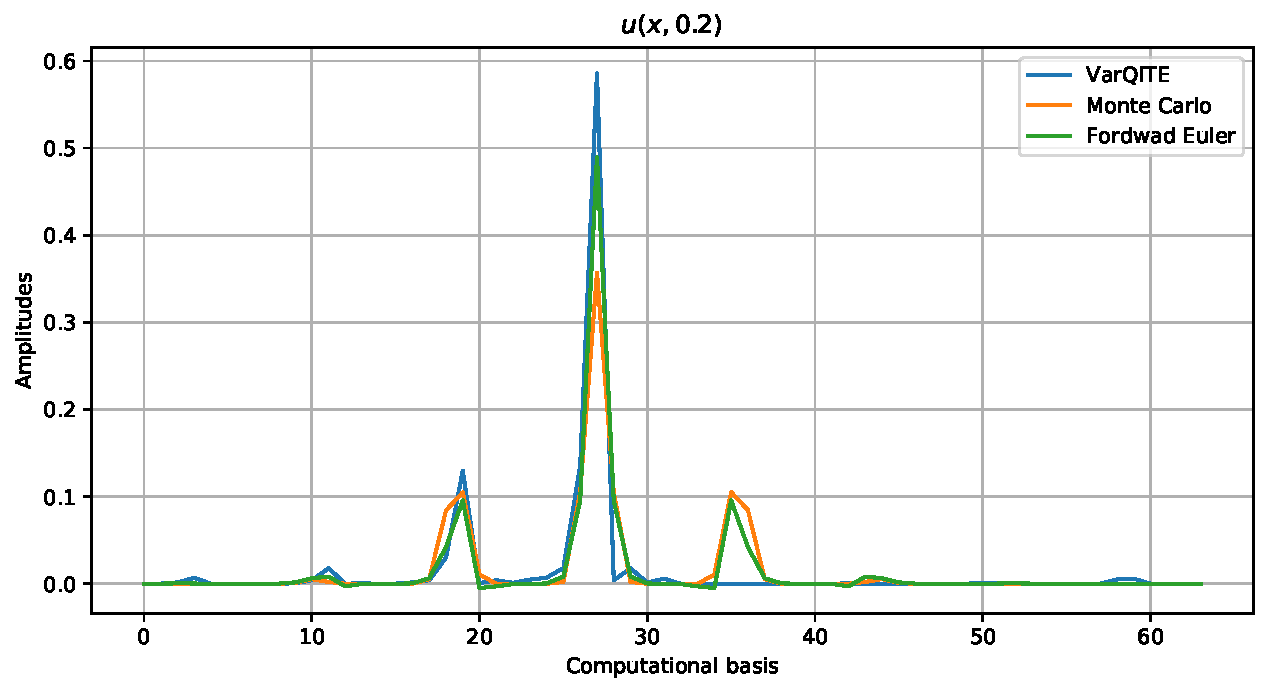
\includegraphics[width=1.0\textwidth]{qresult.pdf}
\caption{\label{fig:frog}Result of the quantum algorithm, taken from \cite{alghassi_variational_2022}.}
\end{figure}



\subsection{Machine learning algorithm}
The first machine learning algorithm\cite{han_solving_2018} to address the problem uses the SDE form of the problem. We will sketch the method. The general idea is to use many realizations of the SDE to generate training data, and approximate a high dimensional function that arose using neural network trained by the previous generated data.
\subsubsection{Deep BSDE}
We want to solve $$
\begin{array}{r}
\partial_t u(t, x)+\frac{1}{2} \sigma \sigma^T(t, x): \nabla^2 u(t, x)+\mu(t, x) \cdot \nabla u(t, x)+f\left(t, x, u(t, x), \sigma^T(t, x) \nabla u(t, x)\right)=0 \\
u(T, x)=g(x)
\end{array}
$$
Consider the SDE
$$
X_t=x+\int_0^t \mu\left(s, X_s\right) d s+\int_0^t \sigma\left(s, X_s\right) d W_s
$$
which directly implies $X_0=x$. The backward SDE associated with this process is
$$
Y_t=g\left(X_T\right)+\int_t^T f\left(s, X_s, Y_s, Z_s\right) d s-\int_t^T Z_s \cdot d W_s,
$$
which in particular implies $Y_T=g\left(X_T\right)$.\\
Under suitable regularity assumptions ,
$$
Y_t=u\left(t, X_t\right) \quad \text { and } \quad Z_t=\left(\sigma^T \nabla u\right)\left(t, X_t\right) \text {. }
$$
Thus, the solution $u(0, x)$ can be obtained through the knowledge of $Y_0=u\left(0, X_0\right)=u(0, x)$.\\

Simulate the SDE in Euler-Maruyama scheme to derive some realizations $\tilde{X}_n$. After that, notice that
$$
\tilde{Y}_{n+1}=\tilde{Y}_n-f\left(t_n, \tilde{X}_n, \tilde{Y}_n, \tilde{Z}_n\right)\left(t_{n+1}-t_n\right)+\tilde{Z}_n \cdot\left(W_{t_{n+1}}-W_{t_n}\right), \quad \tilde{Y}_N=g\left(\tilde{X}_N\right)
$$
indicates that there are multiple unknowns present in this equation, namely
 $\tilde{Y}_0$, an approximation of $u(0, x)$ as well as
 $\tilde{Z}_i$, the approximations of $\sigma^T\left(t_i, \tilde{X}_i\right) \nabla u\left(t_i, \tilde{X}_i\right)$ for $i=0, \ldots, N-1$.
The unknowns $\tilde{Y}_0 \approx u(0, x) \in \mathbb{R}$ and $\tilde{Z}_0 \approx\left(\sigma^T \nabla u\right)(0, x) \in \mathbb{R}^d$ are treated as individual network parameters (we only need both of them in the particular point $(0, x))$ which are learned during training.
To approximate the remaining unknowns $\tilde{Z}_i$ we employ neural networks which realize the mappings $x \mapsto$ $\sigma^T\left(t_i, x\right) \nabla u\left(t_i, x\right)$ for $i=1, \ldots, N$.
These networks have the following structure:
Input $\rightarrow B N \rightarrow$ (Dense $\rightarrow B N \rightarrow$ ReLU) $\rightarrow$ (Dense $\rightarrow B N \rightarrow$ ReLU) $\rightarrow$ Dense $\rightarrow B N \rightarrow$ Output, where  $BN$ stands for batch normalization.

%%%%%%%%%%%%%%%%%%%%%%%%%%%%%%%%%%%%%%%%%%%%%%%%%%%%%%%%%%%%%%%%%%%%%%%%%%%%%%

\section{Discussion}
\paragraph{Curse of dimensionality. }
We have seen from the implementation of the quantum algorithm that whether it overcomes the curse of dimensionality is a complex problem to answer. From the design of the algorithm, its runtime is polynomial in the dimension of the problem and the qubits needed to implement the algorithm scales polynomially with the dimension. This is the necessary condition of overcoming the curse of dimensionality. However, up to now no one has proven the theoretical convergence or a priori error bound on the algorithm, making us unable to claim it overcomes the curse of dimensionality. Both methods perform well empirically, are comparable to the expensive traditional Monte-Carlo method.\\

The major difficulty can come from understanding expressibility of the variational circuit with the design of ansatz, which is not very well known. The expressible states form a low dimensional manifold lying in the very large exponential space, and whether the desried states live near them needs to be investigated.
Both machine learning method and quantum computing method up to now has no satisfactory error control on the problem, and there's a lot of work to be done.\\
\paragraph{Variational quantum circuits and machine learning. }
Variational quantum circuits are in many ways similar to neural-network machine learning. In this algorithm, the updating of the parameters is used by solving an ordinary differential equation instead of using gradient-based method. This is similar to the neural ordinary differential equations\cite{DBLP:journals/corr/abs-1806-07366}, where the authors train the deep Resnets using an ODE solver. \\

Traditional algorithm and machine learning alorithm all uses the SDE form of the problem while quantum algorithm directly uses the PDE form of the problem. Quantum algorithm has the advantage of utilizing shallow circuits, which implies it efficiently uses the parameters. To the contrary, the neural network is heavily over-parameterized and very deep. This implies quantum model can be have less complexity and this may provides robustness. It also avoids the problem of generalization error in machine learning, but expressibility is a question.\\
The problem of quantum algorithm may also be that to simulate very high dimensional equation, one must have a fault-tolerant circuit, the number of qubits scales at least linearly with the dimension, which may face difficulty in terms of hardware. On the contrast, machine learning model can deal with very high dimension as long as sufficient training data is provided. Thus, we are grounded to believe the playground of quantum circuits can be in some middle dimensional problem, say $\sim 10$ or so, which already breaks traditional algorithm. Machine learning, on the other hand, deal with other flexible problems better, like neural operator mapping.  
%%%%%%%%%%%%%%%%%%%%%%%%%%%%%%%%%%%%%%%%%%%%%%%%%%%%%%%%%%%%%%%%%%%%%%%%%%%%%%

\section{Conclusion}
We have explained how to transform a family of  time evolution PDEs into Schrödinger-type equations, make discrete approximation of the problem, use ansatz to create variational circuit, update parameters by solving an ODE, and use suitable quantum embeddings to represent PDE solution. We have discussed extensively the advantage and disadvantage of the algorithm with a comparison of machine learning methods.\\

Lots of future work can be done relevant to the topic. We have not explored other important PDEs and can explore algorithm to solve these equations. Theoretical investigations on error bound, convergence and converge speed is an important topic. Empirically comparing accuracy and speed for different anastz choice are also topic we do not cover. Preservation of certain quantities of the states, like in this problem, the $\ell_1$ norm, is also worth considering as preserving these quantities produce physically meaningful solutions. We believe this is an exciting field for more researchers to put in serious consideration, especially for people in the computational math community.


%%%%%%%%%%%%%%%%%%%%%%%%%%%%%%%%%%%%%%%%%%%%%%%%%%%%%%%%%%%%%%%%%%%%%%%%%%%%%%




%%%%%%%%%%%%%%%%%%%%%%%%%%%%%%%%%%%%%%%%%%%%%%%%%%%%%%%%%%%%%%%%%%%%%%%%%%%%%%
\nocite{*}

\bibliographystyle{siam}
\bibliography{lib}

\end{document}
